% define colors 
\colorlet{fillbottom}{yellow!60}
\colorlet{filltop}{blue!20}
\colorlet{curvecolor}{cyan}
\colorlet{meshcolor}{cyan}

 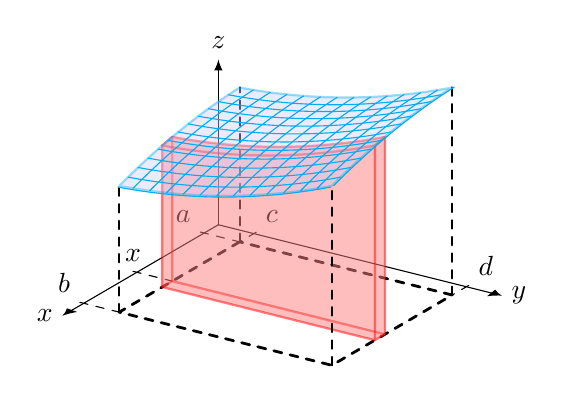
\begin{tikzpicture}[
 %3d view={135}{60},
 x={(-0.6cm,-0.35cm)},z={(0,0.2cm)},y={(1cm,-.25cm)}, 
 %  x={(-0.6cm,-0.5cm)},z={(0,0.2cm)},y={(1cm,-.3cm)}, 
 scale=1.5, line cap=round, line join=round
 ]
% \shorthandoff{:;!?} % https://groups.google.com/g/fr.comp.text.tex/c/K2CEGtgU3YQ
 %===================================
 %  surface 1: z=xy with domain boundary x=1, y=x, y=0
 % surface 2:  z=x^2+y^2 with domain boundary y=x, y=1, x=0
 %===================================
%  \tikzset{
%     declare function={
%         f(\u,\v)=(-(\u/1)^2+(\v/0.8)^2)/3+6.5;
%         }
%     }
\pgfmathdeclarefunction{f}{2}{%
    \pgfmathparse{(-(#1/1)^2+(#2/0.8)^2)/3+6.5}%
}

    \def\l{2}
 
    \def\w{1}
    \def\offset{1/4}
    \def\eps{1/30}
    \def\rad{0.05}

    \def\a{0.2}
    \def\b{1.9}
    \def\c{0.3}
    \def\d{2.1}


    \def\N{10}
    \pgfmathsetmacro{\step}{(\b-\a)/(\N+2)}
    \pgfmathsetmacro{\y}{\c+6*\step}
    \def\ythick{1*\step}

    \def\opacoupe{0.3}

% set coordinates 
     \def \mxmin{0}\def \xdash{0} \def\mxmax{2.5}
     \def \mymin{0}\def \ydash{0} \def\mymax{2}
     \def \mzmin{0}\def \zdash{0} \def\mzmax{2}

%%%%%%%%%%%%%%%%%%%%%%%%%%%%%%%%%%%%
%%%%%%%%%%%%%%%%%%%%%%%%%%%%%%%%%%%%
    \coordinate (O) at (\l*1/2,\l*1/2,0);
    \coordinate (X) at (\l*1/4,\l*1/4,0);
    \coordinate (Y) at ({\l*(1-1/4)},{\l*(1-1/4)},0);    
    
    \draw[line width=\w pt,black, dashed] (\a,\c,0) -- (\b,\c,0) -- (\b,\d,0) -- (\a,\d,0) -- cycle;

    \draw[arrows = {-latex[slant=-0.85]}] (0,0,0)--(\l*1.1,0,0) node[left]{$x$};
    \draw[arrows = {-latex[slant=0.75]}] (0,0,0)--(0,\l*1.2,0) node[right]{$y$};
    \draw[-latex] (0,0,0) -- (0,0,7) node[pos = 1.1] {$z$};
     
%%%%%%%%%%%%%%%%%%%%%%%%%%%%%%%%%%%%
%%%%%%%%%%%%%%%%%%%%%%%%%%%%%%%%%%%%

   \draw[dashed] (\a,-\eps,0)[above left] node {$a$} --(\a,\c,0);
   \draw[dashed] (\b,-\eps,0)[above left] node {$b$} --(\b,\c,0);
   \draw[dashed] (-\eps,\c,0)[above right] node {$c$}--(\a,\c,0);
   \draw[dashed] (-\eps,\d,0)[above right] node {$d$}--(\a,\d,0);

   \draw[dashed] (\y,-\eps,0)[above] node {$x$}--(\y,\c,0);


% help lines
   \draw[thick,dashed] (\a,\c,0)--(\a,\c,{f(\a,\c)});
   \draw[thick,dashed] (\b,\c,0)--(\b,\c,{f(\b,\c)});
   \draw[thick,dashed] (\a,\d,0)--(\a,\d,{f(\a,\d)});
% coupe

\draw[thick,draw=red,fill=red!50!white,opacity=\opacoupe] 
   (\y,\c,0) --
   plot[domain=0:{f(\y,\c)},samples=50,smooth] (\y,\c,\x)
   --
   plot[domain=\c:\d,samples=50,smooth] ({\y},{\x},{f(\y,\x)})
   --
   plot[domain={f(\y,\d)}:0,samples=50,smooth] (\y,\d,\x)
   --
   cycle;
\draw[thick,draw=red,fill=red!50!white,opacity=\opacoupe] 
   (\y,\c,0) -- (\y+\ythick,\c,0) -- (\y+\ythick,\d,0) -- (\y,\d,0) -- cycle;
\draw[thick,draw=red,fill=red!50!white,opacity=\opacoupe] 
   (\y,\c,0) -- (\y+\ythick,\c,0) -- (\y+\ythick,\c,{f(\y+\ythick,\c)}) -- (\y,\c,{f(\y,\c)}) -- cycle;
\draw[thick,draw=red,fill=red!50!white,opacity=\opacoupe] 
   (\y+\ythick,\c,0) --
   plot[domain=0:{f(\y+\ythick,\c)},samples=50,smooth] (\y+\ythick,\c,\x)
   --
   plot[domain=\c:\d,samples=50,smooth] ({\y+\ythick},{\x},{f(\y+\ythick,\x)})
   --
   plot[domain={f(\y+\ythick,\d)}:0,samples=50,smooth] (\y+\ythick,\d,\x)
   --
   cycle;
\draw[thick,draw=red,fill=red!50!white,opacity=\opacoupe] 
   (\y,\d,0) -- (\y+\ythick,\d,0) -- (\y+\ythick,\d,{f(\y+\ythick,\d)}) -- (\y,\d,{f(\y,\d)}) -- cycle;

\draw[thick,draw=red,fill=red!50!white,opacity=\opacoupe] 
   (\y,\c,{f(\y,\c)})--
   plot[domain=\c:\d,samples=50,smooth] ({\y},{\x},{f(\y,\x)})
   --
   plot[variable=\Y,domain=\y:\y+\ythick,samples=50,smooth] ({\Y},\d,{f(\Y,\d)}) 
   --
   plot[domain=\d:\c,samples=50,smooth] (\y+\ythick,\x,{f(\y+\ythick,\x)}) 
   --
   plot[variable=\Y,domain=\y+\ythick:\y,samples=50,smooth] (\Y,\c,{f(\Y,\c)}) 
   --
   cycle;

   
\draw[thick,dashed] (\b,\d,0)--(\b,\d,{f(\b,\d)});

%  surface 1
  \draw[thick,draw=curvecolor,fill=filltop,opacity=0.4] 
   (\a,\c,{f(\a,\c)})--
   plot[domain=\a:\b,samples=50,smooth] ({\x},{\c},{f(\x,\c)})
   --
   plot[variable=\y,domain=\c:\d,samples=50,smooth] (\b,{\y},{f(\b,\y)}) 
   --
   plot[domain=\b:\a,samples=50,smooth] (\x,\d,{f(\x,\d)}) 
   --
   plot[variable=\y,domain=\d:\c,samples=50,smooth] (\a,\y,{f(\a,\y)}) 
   --
   cycle;
   
% surface 1: mesh lines  
\foreach \k [evaluate=\k as \x using \a + \k * \step] in {-1,...,\N} {
    \draw[meshcolor] plot[variable=\y,domain=\c:\d,samples=50,smooth] (\a+\x+0.1,\y,{f(\a+\x+0.1,\y)});
}
\foreach \k [evaluate=\k as \i using \c + \k * \step] in {-2,...,\N} {
    \draw[meshcolor] plot[domain=\a:\b,samples=50,smooth] (\x,\c+\i+0.1,{f(\x,\c+\i+0.1)});
}

 %======================
 \end{tikzpicture}
